\documentclass[tikz,border=10pt]{standalone}
\usepackage{tikz}
\usetikzlibrary{arrows.meta,positioning}

\tikzset{
  card/.style={draw=blue!70!black, line width=1.2pt, rectangle, rounded corners=2pt, minimum width=3.3cm, minimum height=1.4cm, align=center, fill=none},
  signal/.style={->, line width=1.2pt, draw=black!80, >=Stealth}
}

\begin{document}
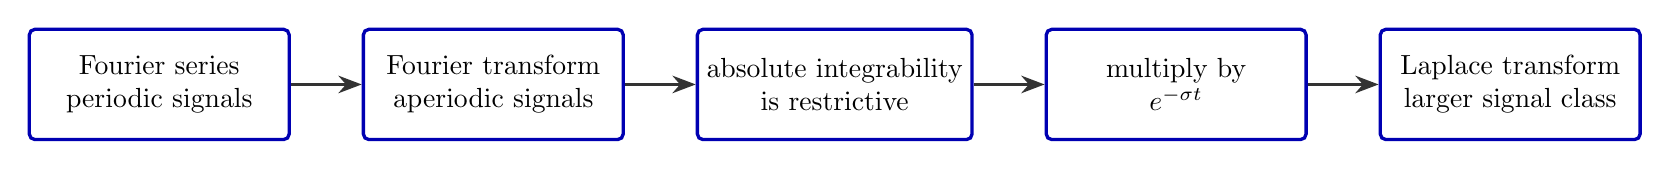
\begin{tikzpicture}[node distance=0.9cm]
  \node[card] (a) {Fourier series\\periodic signals};
  \node[card, right=of a] (b) {Fourier transform\\aperiodic signals};
  \node[card, right=of b] (c) {absolute integrability\\is restrictive};
  \node[card, right=of c] (d) {multiply by\\$e^{-\sigma t}$};
  \node[card, right=of d] (e) {Laplace transform\\larger signal class};
  \draw[signal] (a) -- (b);
  \draw[signal] (b) -- (c);
  \draw[signal] (c) -- (d);
  \draw[signal] (d) -- (e);
\end{tikzpicture}
\end{document}
